% \FloatBarrier
\section{Datasets} \label{sec:res_Datasets}

\subsection{Environment Pre-labeling}

Figure \ref{fig:res_DatasetsPrelabel} attempts to visualize the quality of datasets and labels before the post-labeling process in the data acquisition pipeline is applied. Plots are generated from a small, random subset of samples. They are grouped such that both x- and y-coordinates of gaze can be observed parallel to the XY-dispersion feature, discussed in section \ref{sec:meth_FeatureGeneration}. Since this feature likely will be one of the primary variables to distinguish classes during classification, it serves as a good indicator of the accuracy of labels against the ground truth.

\begin{figure}[h]
    \centering
    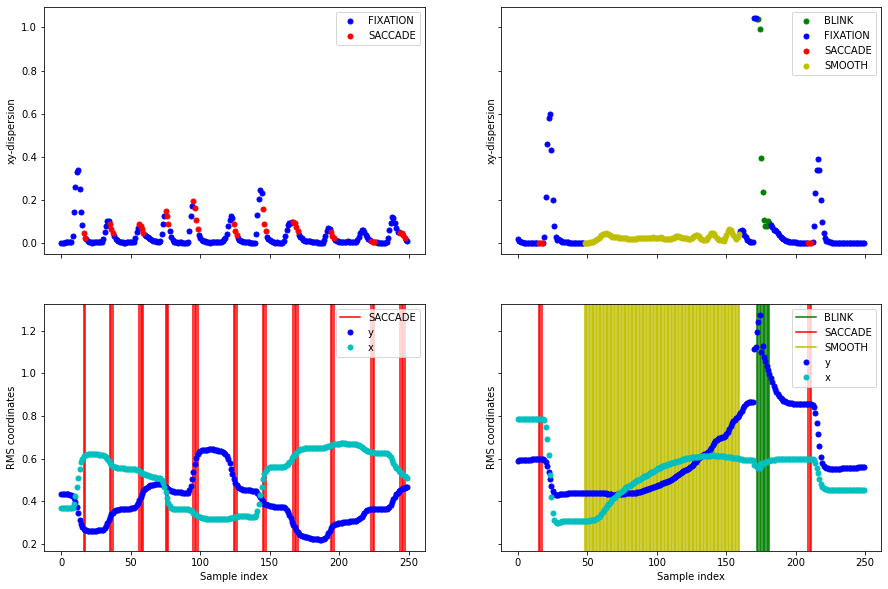
\includegraphics[width=0.8\textwidth]{Images/Dataset/DatasetsPrelabel.png}
    \caption{Dataset as output from static (left) and dynamic (right) recording environments. All plots show individual samples as dots, plotted against the RMS-value of their raw coordinates (bottom) and XY-dispersion (top). Red, green, and yellow samples are color-coded such that dots (top) and vertical lines (bottom) signify samples that are labeled saccades, blinks, and smooth pursuits, respectively. To avoid cluttering, fixations are blue in the top plot and white in the bottom.}
    \label{fig:res_DatasetsPrelabel}
\end{figure}

% \begin{figure}[h]
%     \centering
%     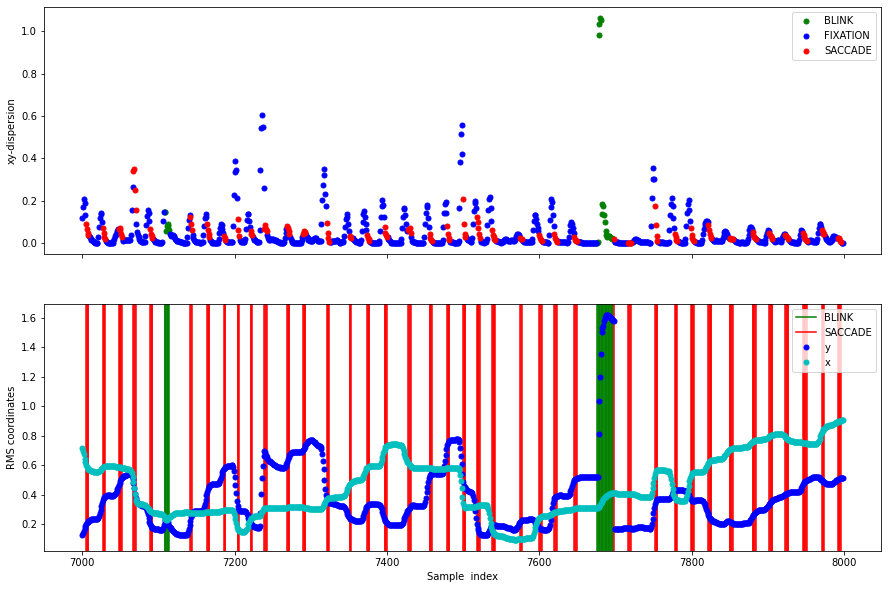
\includegraphics[width=\textwidth]{Images/Dataset/DQ_V1.png}
%     \caption{Dataset from manual user labeling in static environment. The top plot show xy-dispersion and the bottom plot show x-y on-screen coordinates. Both plots are taken form a random subset of 1000 samples in the dataset. Red vertical lines and dots indicate samples where a saccade is labelled, and green vertical lines and dots indicate samples where a blink is labelled. Blue dots are samples labelled as a fixation.}
%     \label{fig:res_HumanErrorBias}
% \end{figure}

% \subsection{Blink event}

\subsection{Final dataset}

Finally, after data has been recorded, imported, processed, and post-labeled, we get the dataset from which the subset presented in figure \ref{fig:res_DatasetFinal} is taken. By comparing this plot to the right one of figure \ref{fig:res_DatasetsPrelabel}, one can observe that they represent the same set of eye-tracking data samples. This dataset is the one that will be utilized to train the final classification model.

\begin{figure}[h]
    \centering
    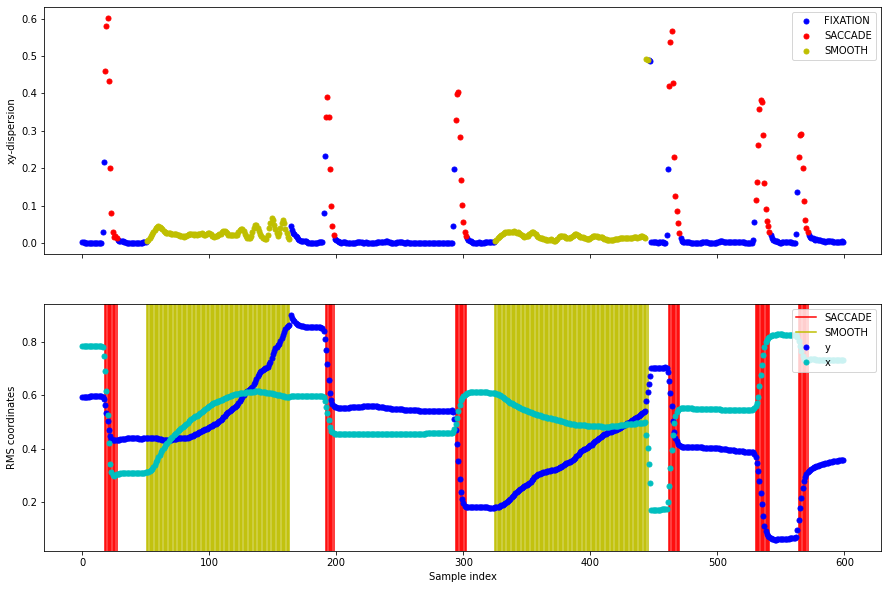
\includegraphics[width=0.8\textwidth]{Images/Dataset/DatasetFinal.png}
    \caption{Final dataset to be used for classification. Axes and labels are identical to that of figure \ref{fig:res_DatasetsPrelabel}.}
    \label{fig:res_DatasetFinal}
\end{figure}

\FloatBarrier